\chapter{Kemantapan Genom: Kerusakan, Perbaikan, dan Rekombinasi DNA}\label{ch:b3:dna-repair}

Satu petang di pantai menanamkan kira-kira seratus ribu \omterm{def:b3:dna-repair:lesions}{lesi} kimia ke dalam
DNA setiap sel kulit yang terpapar matahari: timina bersebelahan yang dilas
menjadi dimer oleh sinar ultraungu, basa yang teroksidasi, untai yang
tertakik. Tanpa matahari sama sekali, air hangat di dalam sel menanggalkan
kira-kira sepuluh ribu purina dari gulanya setiap hari dan mengubah ratusan
sitosina menjadi urasil. Namun laju mutasi sebuah sel manusia hanya sekitar
satu perubahan tiap sepuluh miliar pasangan basa tiap pembelahan --- di dalam
genom berisi enam miliar, kurang dari satu mutasi baru tiap pembelahan.
Jurang antara kerusakan yang diderita sebuah genom dan kerusakan yang
disimpannya ditutup oleh perbaikan: selusin sistem enzim yang meronda heliks
ganda, mengenali apa yang semestinya tidak ada di situ, memotongnya keluar
lalu membangunnya kembali dari untai yang tak rusak, dan, ketika kedua
untainya putus, menyambungnya kembali atau menyalin kepingan yang hilang dari
sebuah saudarinya. Anak-anak yang kekurangan salah satu sistem itu ---
melepuh pada sentuhan cahaya matahari yang pertama, atau terkena kanker usus
besar pada umur tiga puluhan --- memperlihatkan betapa berharganya sistem
tersebut. Bab ini membahas kerusakannya, jalur perbaikannya, permesinan
rekombinasi yang memperbaiki putus yang terparah dan yang dipinjam meiosis,
serta keputusan sel, ketika perbaikannya gagal, untuk berhenti membelah atau
mati.

\section{Apa yang salah pada DNA}

\begin{definition}[Lesi DNA]\label{def:b3:dna-repair:lesions}
\index{lesi DNA}\index{depurinasi}\index{deaminasi}%
\index{dimer pirimidina}\index{putus untai ganda}\index{8-oksoguanina}
Sebuah \emph{lesi} adalah perubahan kimia apa pun pada DNA yang menyimpang
dari keempat basa normal yang berpasangan benar pada tulang punggung yang
utuh. Lesi spontan timbul dari kimia air dan oksigen: \emph{depurinasi},
yakni hidrolisis ikatan antara sebuah purina dan gulanya, yang meninggalkan
tapak tanpa basa (sekitar $10^{4}$ tiap sel tiap hari); \emph{deaminasi},
yang mengubah sitosina menjadi urasil, 5-metilsitosina menjadi timina, dan
adenina menjadi hipoksantina (beberapa ratus tiap hari); \emph{oksidasi} oleh
spesi oksigen reaktif, terutama menjadi \emph{8-oksoguanina}, yang
berpasangan dengan adenina semudah dengan sitosina; serta \emph{galat
replikasi}, yakni basa yang salah disisipkan atau tergelincir. Lesi
lingkungan mencakup \emph{dimer pirimidina siklobutana} dan fotoproduk 6-4
yang dibuat sinar ultraungu di antara dua pirimidina bersebelahan; basa
teralkilasi dari zat pengalkil (O$^{6}$-metil-guanina berpasangan dengan
timina); aduk ruah dari hidrokarbon aromatik dan aflatoksin; taut-silang
antaruntai dari sisplatin dan mustar nitrogen; serta putus untai tunggal dan
\emph{putus untai ganda} yang dibuat radiasi pengion, kira-kira \num{1000}
putus untai tunggal dan \numrange{30}{40} putus untai ganda tiap sel tiap
gray.
\end{definition}

\begin{proposition}[Tangga kesetiaan]\label{prop:b3:dna-repair:fidelity}
\index{kesetiaan}\index{uji baca}\index{perbaikan salah pasang}
Replikasi mencapai laju galatnya sebesar kira-kira $10^{-10}$ tiap pasangan
basa lewat tiga langkah yang berlipat ganda. Pemilihan basa oleh
polimerasenya, berdasarkan geometri dan ikatan hidrogen, meleset kira-kira
sekali tiap $10^{5}$; \emph{\omterm{prop:b3:dna-repair:fidelity}{uji baca}} oleh eksonuklease 3$'\to$5$'$
polimerasenya, yang mengeksisi basa ujung yang salah berpasangan sebelum
pemanjangan, membuang \qty{99}{\%} dari kelesetan itu; \emph{\omterm{prop:b3:dna-repair:fidelity}{perbaikan salah
pasang}}, yang bekerja di belakang garpu pada untai yang baru dibuat, membuang
\qty{99.9}{\%} sisanya. Hasil kali
$10^{-5}\times 10^{-2}\times 10^{-3} = 10^{-10}$ adalah laju teramatinya, dan
cacat pada salah satu langkah pembetulan itu menaikkannya seratus atau seribu
kali lipat: sel semacam itu disebut \emph{mutator}.
\end{proposition}

\begin{example}[Lesi lawan mutasi]\label{ex:b3:dna-repair:numbers}
Sebuah sel manusia berisi $6.4\times 10^{9}$ pasangan basa yang membelah
sekali sehari menimbun sekitar $10^{4}$--$10^{5}$ \omterm{def:b3:dna-repair:lesions}{lesi} tiap hari dan
sekitar $6.4\times 10^{9}\times 10^{-10} \approx 0.6$ mutasi baru tiap
pembelahan: kurang dari satu \omterm{def:b3:dna-repair:lesions}{lesi} dari sepuluh ribu yang bertahan menjadi
perubahan yang tetap. Sisanya diperbaiki sebelum replikasi membacanya, dan
laju bertahannya \omterm{def:b3:dna-repair:lesions}{lesi} menjadi mutasi --- bukan laju kerusakannya --- itulah
yang diperkecil oleh seleksi. Aritmetika yang sama memperlihatkan mengapa
cacah mutasi di dalam sebuah tumor atau di dalam sperma seorang ayah yang
lebih tua sesungguhnya menghitung pembelahan: mutasi yang diusung sebuah sel
kira-kira sama dengan cacah pembelahan yang dilaluinya dikali galat tiap
pembelahan.
\end{example}

\section{Perbaikan satu untai yang rusak}

\begin{definition}[Perbaikan eksisi]\label{def:b3:dna-repair:excision}
\index{perbaikan eksisi basa}\index{perbaikan eksisi nukleotida}%
\index{glikosilase}\index{xeroderma pigmentosum}
Sebagian besar \omterm{def:b3:dna-repair:lesions}{lesi} mengenai satu untai dan diperbaiki dengan memotong
keping yang rusak lalu menyalin untai yang lain. \emph{Perbaikan eksisi basa}
(BER) menangani \omterm{def:b3:dna-repair:lesions}{lesi} kecil yang tidak merusak bentuk: sebuah \emph{glikosilase
DNA} yang khas bagi satu macam basa yang salah (glikosilase urasil-DNA,
glikosilase 8-oksoG, dan beberapa lainnya) membalikkan basa itu ke luar
heliks lalu memotongnya dari gulanya; sebuah endonuklease AP menakik tulang
punggungnya pada tapak tanpa basa itu; sebuah polimerase (Pol~$\beta$)
membuang gulanya lalu menyisipkan satu nukleotida; sebuah ligase menutupnya.
\emph{Perbaikan eksisi nukleotida} (NER) menangani \omterm{def:b3:dna-repair:lesions}{lesi} ruah yang merusak
bentuk heliks --- \omterm{def:b3:dna-repair:lesions}{dimer pirimidina}, aduk kimia --- tanpa mengenali kimia \omterm{def:b3:dna-repair:lesions}{lesi}
itu sendiri: kerusakan bentuknya dideteksi (oleh XPC yang memindai genom, atau
oleh RNA polimerase yang terhenti pada cabang yang terkopel transkripsi),
heliksnya dibuka oleh subunit helikase TFIIH, kerusakannya diverifikasi (XPA),
dua endonuklease (XPF, XPG) memotong untai yang rusak pada jarak
\numrange{24}{32} nukleotida, oligonukleotidanya dilepaskan, lalu polimerase
dan ligase mengisi celahnya. Hilangnya salah satu dari ketujuh protein XP
menimbulkan \emph{xeroderma pigmentosum}: kepekaan luar biasa terhadap cahaya
matahari, bintik cokelat, dan laju kanker kulit yang seribu kali lipat lebih
tinggi.
\end{definition}

\begin{proof}[Bukti eksperimental]
Cleaver (1968) membiakkan fibroblas kulit pasien \omterm{def:b3:dna-repair:excision}{xeroderma pigmentosum},
menyinarinya dengan cahaya ultraungu, lalu memberinya timidina radioaktif di
luar fase S. Sel normal memasukkan labelnya pada banyak tapak kecil --- yaitu
``sintesis DNA tak terjadwal'' berupa tambalan perbaikan --- sedangkan sel
pasiennya hampir tidak memasukkan apa pun, dan mati pada dosis yang masih
dilewati sel normal: penyakitnya adalah kegagalan mengeksisi dimernya.
Menggabungkan sel dua pasien sering memulihkan perbaikannya pada sel hibrid,
karena masing-masing memasok apa yang tidak dimiliki yang lain; dengan uji itu
para pasien dipilah menjadi golongan komplementasi A sampai G, satu golongan
tiap gen jalurnya, bertahun-tahun sebelum gennya diklon.
\end{proof}

\begin{omfigure}
\begin{tikzpicture}[every node/.style={font=\scriptsize}, >=stealth]
  % BER column
  \node[font=\small\bfseries] at (2.0,3.2) {Perbaikan eksisi basa};
  \foreach \y/\txt in {2.6/{basa rusak (U, 8-oksoG)}, 1.5/{glikosilase membuang basanya}, 0.4/{endonuklease AP menakik}, -0.7/{Pol $\beta$ mengisi satu nukleotida, ligase menutup}} {
    \draw[very thick, omDef] (0.2,\y) -- (3.8,\y); \draw[very thick, omDef] (0.2,\y-0.25) -- (3.8,\y-0.25);
    \node[right, align=left] at (0.2,\y-0.6) {\txt};
  }
  \fill[omThm] (2.0,2.6) circle (0.1);
  \draw[omThm, thick] (1.9,1.5) -- (2.1,1.5);
  \draw[white, very thick] (1.9,0.4) -- (2.1,0.4);
  \fill[omMeth!80!black] (2.0,-0.7) circle (0.1);
  % NER column
  \node[font=\small\bfseries] at (8.0,3.2) {Perbaikan eksisi nukleotida};
  \foreach \y/\txt in {2.6/{lesi ruah merusak bentuk heliks; XPC mengikat}, 1.5/{TFIIH membuka heliksnya, XPA memverifikasi}, 0.4/{XPF dan XPG memotong berjarak 24--32 nt}, -0.7/{polimerase mengisi celahnya, ligase menutup}} {
    \draw[very thick, omDef] (6.2,\y) -- (9.8,\y); \draw[very thick, omDef] (6.2,\y-0.25) -- (9.8,\y-0.25);
    \node[right, align=left] at (6.2,\y-0.6) {\txt};
  }
  \draw[omThm, very thick] (7.8,2.6) -- (8.2,2.6) -- (8.2,2.75) -- (7.8,2.75) -- cycle;
  \draw[omDef, very thick] (7.2,1.5) .. controls (7.6,1.85) and (8.4,1.85) .. (8.8,1.5); \draw[omThm, very thick] (7.85,1.72) -- (8.15,1.72);
  \draw[very thick, white] (7.0,0.4) -- (9.0,0.4); \draw[omThm, thick, ->] (7.0,0.7) -- (7.0,0.48); \draw[omThm, thick, ->] (9.0,0.7) -- (9.0,0.48);
  \draw[very thick, omMeth!80!black] (7.0,-0.7) -- (9.0,-0.7);
\end{tikzpicture}

{\small Dua jalur eksisi. Eksisi basa (kiri) mengenali satu basa salah
tertentu dengan \omterm{def:b3:dna-repair:excision}{glikosilase} khusus lalu mengganti satu
nukleotida. Eksisi nukleotida (kanan) mengenali kerusakan bentuk yang
ditimbulkan \omterm{def:b3:dna-repair:lesions}{lesi} ruah mana pun, memotong untainya pada kedua sisi, lalu
mengganti tambalan sepanjang kira-kira tiga puluh nukleotida (hijau).}
\end{omfigure}

\begin{definition}[Perbaikan salah pasang]\label{def:b3:dna-repair:mmr}
\index{perbaikan salah pasang!pembedaan untai}\index{sindrom Lynch}%
\index{ketakmantapan mikrosatelit}
\emph{\omterm{prop:b3:dna-repair:fidelity}{Perbaikan salah pasang}} (MMR) membetulkan pasangan yang keliru dan
lengkung sisipan--delesi kecil yang lolos dari \omterm{prop:b3:dna-repair:fidelity}{uji baca}. Protein MutS
(MSH2--MSH6 pada manusia) mengenali kerusakan bentuk sebuah salah pasang dan,
bersama MutL (MLH1--PMS2), memberi izin kepada sebuah eksonuklease untuk
menguraikan untai yang baru disintesis, dari sebuah takik terdekat sampai
melewati salah pasangnya; celahnya diisi kembali oleh polimerase. Kesulitannya
adalah \emph{pembedaan untai}: sebuah salah pasang memiliki dua basa dan hanya
satu yang keliru. Pada \emph{Escherichia coli} untai barunya dikenali karena
belum termetilasi pada tapak GATC, yang ditandai metilase Dam beberapa menit
sesudah sintesisnya; MutH menakik untai yang tak termetilasi itu. Pada
eukariot untai barunya dikenali dari takik di antara fragmen Okazaki dan dari
ujung 3$'$ bebas untai pengarah. Hilangnya MMR menaikkan laju mutasi seratus
sampai seribu kali lipat, paling kasatmata pada \emph{mikrosatelit} --- deretan
ulangan pendek tempat polimerasenya tergelincir --- yang panjangnya berubah
dari sel ke sel: \emph{ketakmantapan mikrosatelit}. Hilangnya satu alel MMR
secara turunan disebut \emph{sindrom Lynch}, dengan kanker kolorektal pada
sekitar \qty{70}{\%} pembawanya, kerap sebelum umur lima puluh.
\end{definition}

\begin{omfigure}
\begin{tikzpicture}[every node/.style={font=\scriptsize}, >=stealth]
  \draw[very thick, omDef] (0,1.2) -- (9,1.2); \node[left] at (-0.1,1.2) {untai cetakan};
  \draw[very thick, gray] (0,0.6) -- (9,0.6); \node[left] at (-0.1,0.6) {untai baru};
  % methyl groups on template at GATC
  \foreach \x in {1.5,7.5} { \fill[omMeth!80!black] (\x,1.35) circle (0.1); \node[above] at (\x,1.45) {CH$_3$ pada GATC}; }
  \foreach \x in {1.5,7.5} { \draw[omMeth!80!black] (\x,0.45) circle (0.1); }
  \node[below] at (7.5,0.32) {belum termetilasi};
  % mismatch
  \draw[omThm, very thick] (4.5,1.05) -- (4.5,0.75); \node[omThm, right] at (4.6,0.9) {salah pasang};
  \draw[thick, fill=omExo!35] (4.5,1.9) ellipse (1.0 and 0.3); \node at (4.5,1.9) {MutS/MutL};
  \draw[->, thick] (4.5,1.65) -- (4.5,1.3);
  % MutH nick on new strand at unmethylated GATC
  \draw[omThm, thick, ->] (1.5,-0.55) -- (1.5,0.42); \node[omThm, below] at (1.5,-0.55) {MutH menakik untai yang tak termetilasi};
  % excision arrow
  \draw[->, very thick, omProp] (1.7,-0.1) -- (5.0,-0.1); \node[omProp, below] at (3.95,-0.15) {eksonuklease menguraikan sampai melewati salah pasangnya};
  \node[right] at (5.4,-0.8) {lalu Pol III mengisi celahnya, ligase menutupnya};
\end{tikzpicture}

{\small Pembedaan untai pada \omterm{prop:b3:dna-repair:fidelity}{perbaikan salah pasang} bakteri. Untai
cetakannya mengusung gugus metil pada tapak GATC-nya; untai barunya belum,
dan MutH menakiknya di situ. Basa yang keliru karena itu selalu dibuang dari
untai yang baru.}
\end{omfigure}

\begin{method}[Memilah penyakit perbaikan menjadi gen]\label{met:b3:dna-repair:complementation}
\index{uji komplementasi}
Untuk mengetahui berapa gen yang terlibat pada sebuah fenotipe resesif,
sebelum satu gen pun dikenal: (1) ambillah galur sel dari pasien yang tak
berkerabat, yang masing-masing mutan pada suatu gen jalurnya; (2) gabungkanlah
pasangan galur menjadi sel hibrid; (3) ujilah hibridnya untuk fungsi tersebut
(di sini, sintesis DNA tak terjadwal sesudah cahaya ultraungu); (4) bila
hibridnya pulih, kedua pasien itu membawa mutasi pada gen yang \emph{berbeda}
(masing-masing memasok protein yang tak dimiliki yang lain: keduanya
\emph{saling melengkapi}); bila tidak, pada gen yang sama; (5) kelompokkanlah
pasiennya menjadi golongan komplementasi --- satu golongan tiap gen. Cacah
golongannya adalah batas bawah cacah gennya.
\end{method}

\section{Perbaikan kromosom yang putus}

\begin{definition}[Perbaikan putus untai ganda]\label{def:b3:dna-repair:dsb}
\index{penyambungan ujung tak homolog}\index{rekombinasi homolog}%
\index{Rad51}\index{sambungan Holliday}\index{BRCA}
Sebuah \emph{\omterm{def:b3:dna-repair:lesions}{putus untai ganda}} memenggal kromosomnya dan tidak meninggalkan
untai utuh untuk disalin. Dua jalur memperbaikinya. \emph{Penyambungan ujung
tak homolog} (NHEJ): cincin Ku70--Ku80 mengikat tiap ujung, merekrut kinase
DNA-PKcs, nuklease merapikan tonjolannya, lalu ligase IV menyambungkan
ujungnya; jalur ini bekerja pada tahap daur mana pun dan dalam hitungan menit,
tetapi menghilangkan atau menambahkan beberapa nukleotida pada sambungannya
dan dapat menyambungkan ujung yang keliru. \emph{Rekombinasi homolog} (HR):
kompleks MRN dan nuklease memangkas untai 5$'$-nya sehingga tersisa ekor
beruntai tunggal 3$'$ yang panjang, yang diselimuti RPA lalu, dengan bantuan
BRCA2, oleh rekombinase \emph{Rad51}; filamen Rad51 itu mencari duplek yang
homolog --- kromatid saudari, pada fase S dan G2 --- menyerbunya, dan ujung
3$'$ penyerbunya memulai sintesis pada salinan yang utuh. Molekul gabungannya
dapat dibubarkan sesudah sintesis pendek (kebanyakan perbaikan mitosis, tanpa
pertukaran DNA di sisinya) atau matang menjadi dua \emph{sambungan Holliday}
berlengan empat, yang penyelesaiannya oleh endonuklease memberi hasil berupa
pindah silang atau bukan pindah silang. HR bersifat saksama karena ia menyalin
saudari, tetapi hanya tersedia ketika ada saudari.
\end{definition}

\begin{omfigure}
\begin{tikzpicture}[every node/.style={font=\scriptsize}, >=stealth]
  % break
  \draw[very thick, omDef] (0,3.2) -- (2.3,3.2); \draw[very thick, omDef] (2.7,3.2) -- (5,3.2);
  \draw[very thick, omDef] (0,3.0) -- (2.3,3.0); \draw[very thick, omDef] (2.7,3.0) -- (5,3.0);
  \node[above] at (2.5,3.3) {putus untai ganda};
  % NHEJ left
  \draw[->, thick] (1.2,2.8) -- (-0.5,2.0); \node[left, align=right] at (-0.6,2.4) {fase mana pun,\\beberapa menit};
  \node[font=\small\bfseries] at (-1.6,1.55) {NHEJ};
  \draw[thick, fill=omExo!35] (-2.6,0.9) ellipse (0.3 and 0.2); \draw[thick, fill=omExo!35] (-0.8,0.9) ellipse (0.3 and 0.2);
  \draw[very thick, omDef] (-3.4,0.9) -- (-2.9,0.9); \draw[very thick, omDef] (-0.5,0.9) -- (0.0,0.9);
  \node[below] at (-1.7,0.7) {Ku mengikat kedua ujung, perapian};
  \draw[->, thick] (-1.7,0.3) -- (-1.7,-0.1);
  \draw[very thick, omDef] (-3.4,-0.4) -- (0.0,-0.4); \draw[omThm, very thick] (-1.85,-0.4) -- (-1.55,-0.4);
  \node[below, align=center] at (-1.7,-0.55) {ligase IV menyambung:\\beberapa nukleotida hilang atau bertambah};
  % HR right
  \draw[->, thick] (3.8,2.8) -- (5.5,2.0); \node[right, align=left] at (5.6,2.4) {S/G2, ada sebuah\\saudari; beberapa jam};
  \node[font=\small\bfseries] at (6.8,1.55) {HR};
  % resected ends
  \draw[very thick, omDef] (4.6,0.9) -- (6.2,0.9); \draw[very thick, omDef] (7.4,0.9) -- (9.0,0.9);
  \draw[very thick, omDef] (4.6,0.7) -- (5.6,0.7); \draw[very thick, omDef] (8.0,0.7) -- (9.0,0.7);
  \foreach \x in {5.7,5.9,6.1} \fill[omProp] (\x,0.9) circle (0.07);
  \node[below] at (6.8,0.55) {pemangkasan 5$'$; Rad51 menyelimuti ekor 3$'$};
  \draw[->, thick] (6.8,0.15) -- (6.8,-0.25);
  % strand invasion of sister
  \draw[very thick, omMeth!70!black] (4.6,-0.9) -- (9.0,-0.9); \draw[very thick, omMeth!70!black] (4.6,-1.1) -- (9.0,-1.1);
  \draw[very thick, omDef] (4.6,-0.5) -- (5.8,-0.5) .. controls (6.2,-0.5) and (6.3,-0.9) .. (6.6,-0.9) -- (7.6,-0.9);
  \draw[->, omDef, thick] (7.6,-0.9) -- (8.1,-0.9);
  \node[below, align=center] at (6.8,-1.2) {penyerbuan saudarinya (hijau), sintesis pada salinan yang utuh,\\lalu pembubaran (tanpa pindah silang) atau sambungan Holliday};
\end{tikzpicture}

{\small Dua nasib sebuah \omterm{def:b3:dna-repair:lesions}{putus untai ganda}. Kiri: penyambungan ujung,
cepat dan selalu tersedia, dengan ongkos berupa perubahan kecil pada
sambungannya. Kanan: \omterm{def:b3:dna-repair:dsb}{rekombinasi homolog}, yang memangkas ujungnya,
menyerbu kromatid saudari dengan filamen \omterm{def:b3:dna-repair:dsb}{Rad51}, lalu menyalin apa yang
hilang.}
\end{omfigure}

\begin{theorem}[Muatan kerusakan, laju perbaikan, dan garpunya]\label{thm:b3:dna-repair:load}
\index{kerusakan sisa}\index{jalur yang bersaing}
Misalkan \omterm{def:b3:dna-repair:lesions}{lesi} satu macam timbul dengan laju tetap $D$ tiap sel tiap
jam dan dibuang oleh perbaikan orde satu dengan tetapan laju $k$
(waktu paruh $t_{1/2} = \ln 2/k$). Cacah \omterm{def:b3:dna-repair:lesions}{lesi} $L(t)$ memenuhi
$\mathrm{d}L/\mathrm{d}t = D - kL$, sehingga pada keadaan tunak
\[
L^{*} = \frac{D}{k},
\]
dan denyut berisi $N$ \omterm{def:b3:dna-repair:lesions}{lesi} yang diberikan pada $t = 0$ meninggalkan
$N e^{-kT}$ \omterm{def:b3:dna-repair:lesions}{lesi} ketika garpu replikasi tiba pada waktu $T$. Bila dua jalur
bersaing memperebutkan \omterm{def:b3:dna-repair:lesions}{lesi} yang sama dengan tetapan laju $k_{1}$ dan
$k_{2}$, tiap \omterm{def:b3:dna-repair:lesions}{lesi} diperbaiki oleh jalur pertama dengan peluang $k_{1}/(k_{1} +
k_{2})$ dan waktu paruh keseluruhannya $\ln 2/(k_{1} + k_{2})$. Cacah
\omterm{def:b3:dna-repair:lesions}{lesi} yang mencapai garpunya tersebar Poisson dengan rata-rata
$N e^{-kT}$, sehingga peluang bahwa tak satu pun mencapainya adalah $\exp(-N e^{-kT})$.
\end{theorem}
\begin{proof}
Keadaan tunaknya adalah tempat $D = kL$. Untuk denyutnya, $D = 0$ dan
persamaannya terintegralkan menjadi $L = N e^{-kt}$. Dengan dua jalur, laju
kehilangannya adalah $(k_{1} + k_{2})L$; di dalam selang pendek mana pun
sebuah \omterm{def:b3:dna-repair:lesions}{lesi} tertentu dibuang oleh jalur~1 dengan peluang $k_{1}\,\mathrm{d}t$
dan oleh jalur~2 dengan $k_{2}\,\mathrm{d}t$, sehingga peluang bersyarat bahwa
pembuangannya, ketika terjadi, dikerjakan jalur~1 adalah $k_{1}/(k_{1} +
k_{2})$. \omterm{def:b3:dna-repair:lesions}{Lesi} yang saling bebas, yang masing-masing bertahan dengan peluang
$e^{-kT}$, memberi cacah binomial, yang menjadi Poisson pada limit \omterm{def:b3:dna-repair:lesions}{lesi} yang
banyak dan ketahanan yang kecil, dan peluang Poisson untuk nol adalah
$e^{-\text{rata-rata}}$.
\end{proof}

\begin{example}[Mengapa xeroderma adalah penyakit garpu replikasi]\label{ex:b3:dna-repair:xp}
Sebuah dosis matahari meninggalkan $N = 10^{5}$ \omterm{def:b3:dna-repair:lesions}{dimer pirimidina} di dalam
keratinosit. Dengan waktu paruh eksisi nukleotida \qty{2}{h} ($k =
\qty{0.35}{h^{-1}}$) dan garpu yang tiba sesudah \qty{8}{h}, $N e^{-kT} =
10^{5}\times e^{-2.8} \approx 6000$ dimer masih ada untuk disalin; dengan
perbaikan sel XP yang nyaris nihil ($k \approx
\qty{0.01}{h^{-1}}$), tersisa \num{92000}. Tiap dimer yang dijumpai garpunya
dilangkahi oleh \omterm{def:b3:dna-repair:tls}{sintesis lintas lesi} (di bawah), yang rawan galat: muatan
mutasi pasiennya tiap pembelahan lima belas kali lipat muatan yang normal,
dan kanker kulitnya menyusul semasa kanak-kanak. Penyembuhan yang berhasil
adalah menjaga $N$ tetap kecil --- menghindari cahaya ultraungu sama sekali.
\end{example}

\begin{omfigure}
\begin{tikzpicture}
\begin{axis}[
  width=0.7\linewidth, height=5.6cm,
  axis x line=bottom, axis y line=left,
  xmin=0, xmax=12, ymin=100, ymax=200000, ymode=log,
  xlabel={jam sesudah paparan}, ylabel={dimer tiap sel},
  xlabel style={font=\small, at={(axis description cs:0.5,-0.12)}, anchor=north},
  ylabel style={font=\small},
  tick label style={font=\small}, xtick={0,2,4,6,8,10,12},
  clip=false,
]
\addplot[very thick, omDef, domain=0:12, samples=40] {100000*exp(-0.35*x)};
\addplot[very thick, omThm, domain=0:12, samples=40] {100000*exp(-0.01*x)};
\addplot[dashed, gray] coordinates {(8,100) (8,200000)};
\node[font=\scriptsize, anchor=south east, gray] at (axis cs:8,110) {garpu tiba};
\node[font=\scriptsize, omDef, anchor=north east] at (axis cs:11.5,18000) {normal, $t_{1/2} = \qty{2}{h}$};
\node[font=\scriptsize, omThm, anchor=south west] at (axis cs:2,105000) {xeroderma pigmentosum};
\fill[omDef] (axis cs:8,6070) circle (2pt); \node[font=\scriptsize, omDef, anchor=west] at (axis cs:8.3,6070) {\num{6000}};
\fill[omThm] (axis cs:8,92300) circle (2pt); \node[font=\scriptsize, omThm, anchor=north west] at (axis cs:8.3,80000) {\num{92000}};
\end{axis}
\end{tikzpicture}

{\small Dimer yang tersisa sesudah denyut berisi $10^{5}$, pada skala
logaritmik, bagi sel normal dan bagi sel yang eksisi nukleotidanya cacat.
Garpu pada \qty{8}{h} berjumpa dengan \omterm{def:b3:dna-repair:lesions}{lesi} lima belas kali lebih banyak di
dalam sel pasiennya.}
\end{omfigure}

\begin{proof}[Bukti eksperimental]
Holliday (1964) mengusulkan sambungan berlengan empat untuk menjelaskan
teka-teki genetika fungi: pada sebuah persilangan, sebuah tetrad spora
kadang-kadang memperlihatkan pemilahan penanda $3{:}1$, bukan $2{:}2$ menurut
Mendel, dan selalu bagi penanda yang dekat dengan pindah silang. Modelnya ---
pertukaran untai tunggal antara dua duplek homolog, yang membentuk
heterodupleks yang lalu ``dibetulkan'' \omterm{prop:b3:dna-repair:fidelity}{perbaikan salah pasang} ke satu arah
atau arah yang lain (\emph{konversi gen}) --- menjelaskan sekaligus nisbah
yang ganjil itu dan kaitannya dengan pindah silang. Sambungannya sendiri
kemudian terlihat di mikroskop elektron pada plasmid yang berekombinasi dan
di dalam struktur resolvase RuvC yang terikat padanya.
\end{proof}

\section{Toleransi, tanda bahaya, dan keputusan untuk berhenti}

\begin{definition}[Sintesis lintas lesi]\label{def:b3:dna-repair:tls}
\index{sintesis lintas lesi}\index{polimerase eta}
Ketika sebuah garpu berjumpa dengan \omterm{def:b3:dna-repair:lesions}{lesi} yang belum diperbaiki, polimerase
replikatifnya terhenti. \emph{Sintesis lintas \omterm{def:b3:dna-repair:lesions}{lesi}} (TLS) memanggil
polimerase khusus yang tapak aktifnya lebih lapang dan tanpa \omterm{prop:b3:dna-repair:fidelity}{uji baca} ---
Pol~$\eta$ bagi \omterm{def:b3:dna-repair:lesions}{dimer pirimidina}, Pol~$\iota$, $\kappa$, $\zeta$, dan Rev1
bagi \omterm{def:b3:dna-repair:lesions}{lesi} lain --- yang menyisipkan beberapa nukleotida berhadapan dengan
\omterm{def:b3:dna-repair:lesions}{lesinya} lalu menyingkir. Pol~$\eta$ menaruh dua adenina berhadapan dengan
dimer timina, dan itu biasanya benar; yang lain sering keliru. TLS menukar
kesaksamaan demi bertahannya garpu, dan merupakan sumber sebagian besar
mutasi yang diimbas ultraungu. Bentuk varian \omterm{def:b3:dna-repair:excision}{xeroderma pigmentosum} (XP-V)
memiliki perbaikan eksisi yang utuh tetapi tak memiliki Pol~$\eta$: dimer
yang lolos dari eksisi dilangkahi polimerase yang lebih rawan galat, lalu
kankernya menyusul.
\end{definition}

\begin{proposition}[Tanggapan SOS bakteri]\label{prop:b3:dna-repair:sos}
\index{tanggapan SOS}\index{RecA}\index{LexA}
Pada \emph{E.~coli} rekombinase RecA, yang terikat pada DNA beruntai tunggal
yang menumpuk pada garpu terhenti dan putus terpangkas, menjadi koprotease
yang mendorong penekan LexA memotong dirinya sendiri. LexA menekan sekitar
empat puluh gen; seiring turunnya LexA, gen itu dinyalakan berurutan menurut
kegemaran operatornya: mula-mula gen perbaikan eksisi \emph{uvrA} dan
\emph{uvrB}, lalu \emph{recA} sendiri dan penghambat pembelahan sel
\emph{sulA} (selnya berhenti membelah lalu tumbuh menjadi filamen), dan
terakhir polimerase rawan galat Pol~IV dan Pol~V, yang melangkahi \omterm{def:b3:dna-repair:lesions}{lesi} dengan
ongkos berupa mutasi. Tanggapan bertingkat itu mencoba perbaikan yang saksama
lebih dulu dan toleransi mutagenik hanya ketika kerusakannya bertahan; mutasi
yang diimbasnya adalah bahan mentah tempat kekebalan antibiotik berevolusi di
bawah pengobatan.
\end{proposition}

\begin{omfigure}
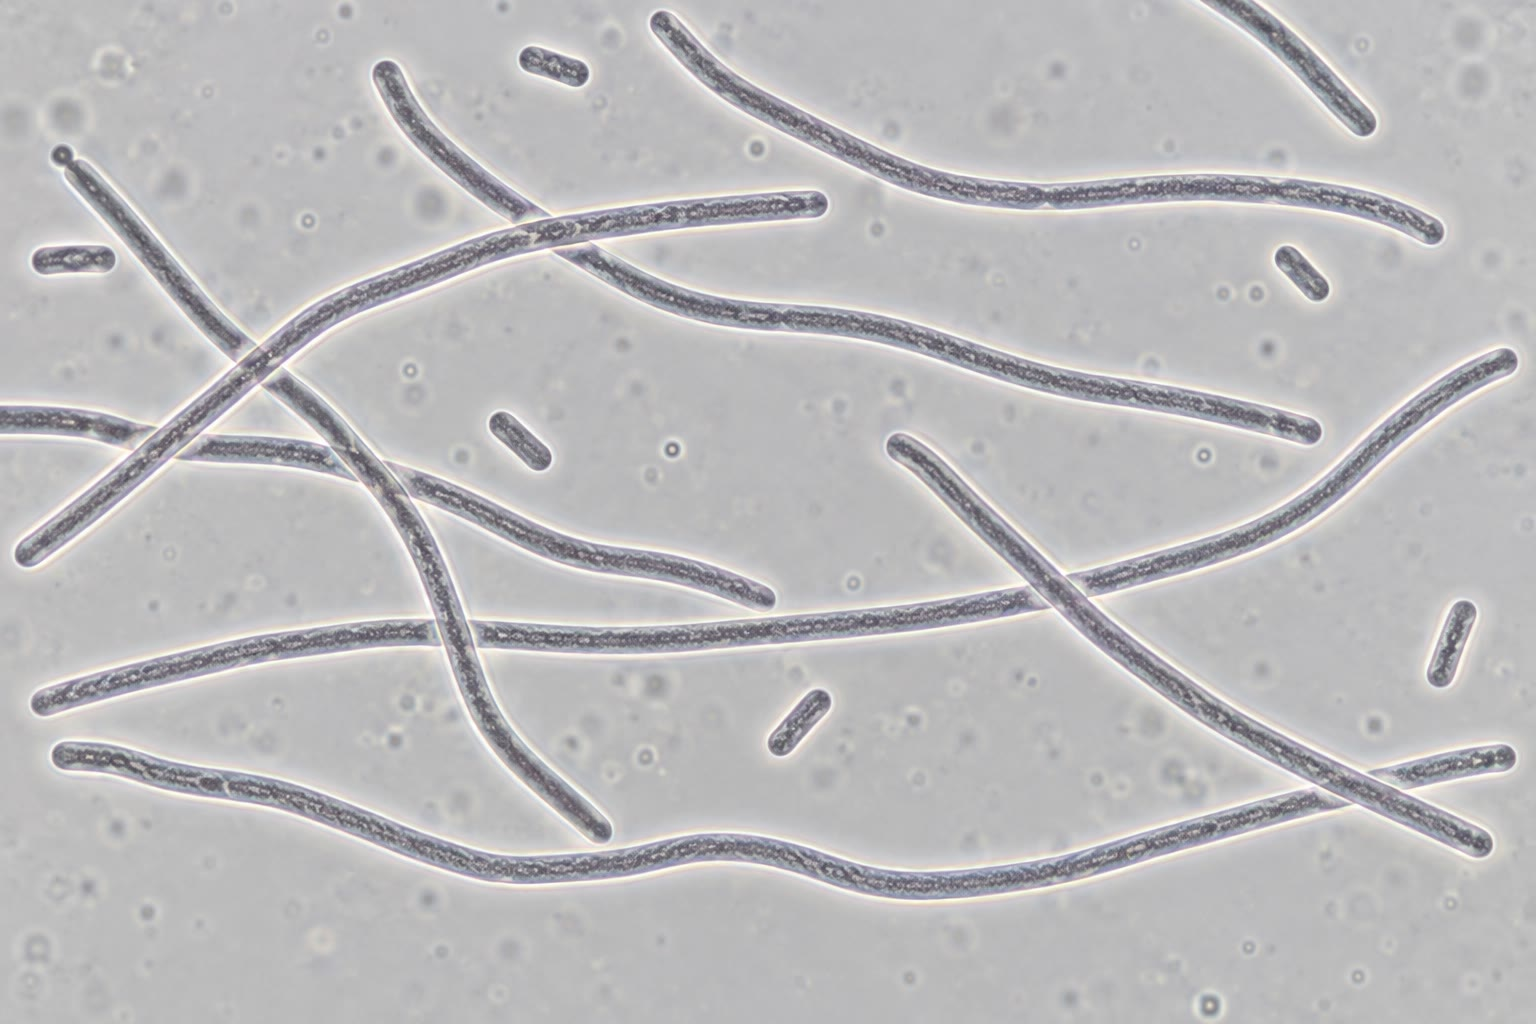
\includegraphics[width=0.46\linewidth]{images/book5/ai/b5-03-sos-filaments.jpg}\hspace{0.04\linewidth}
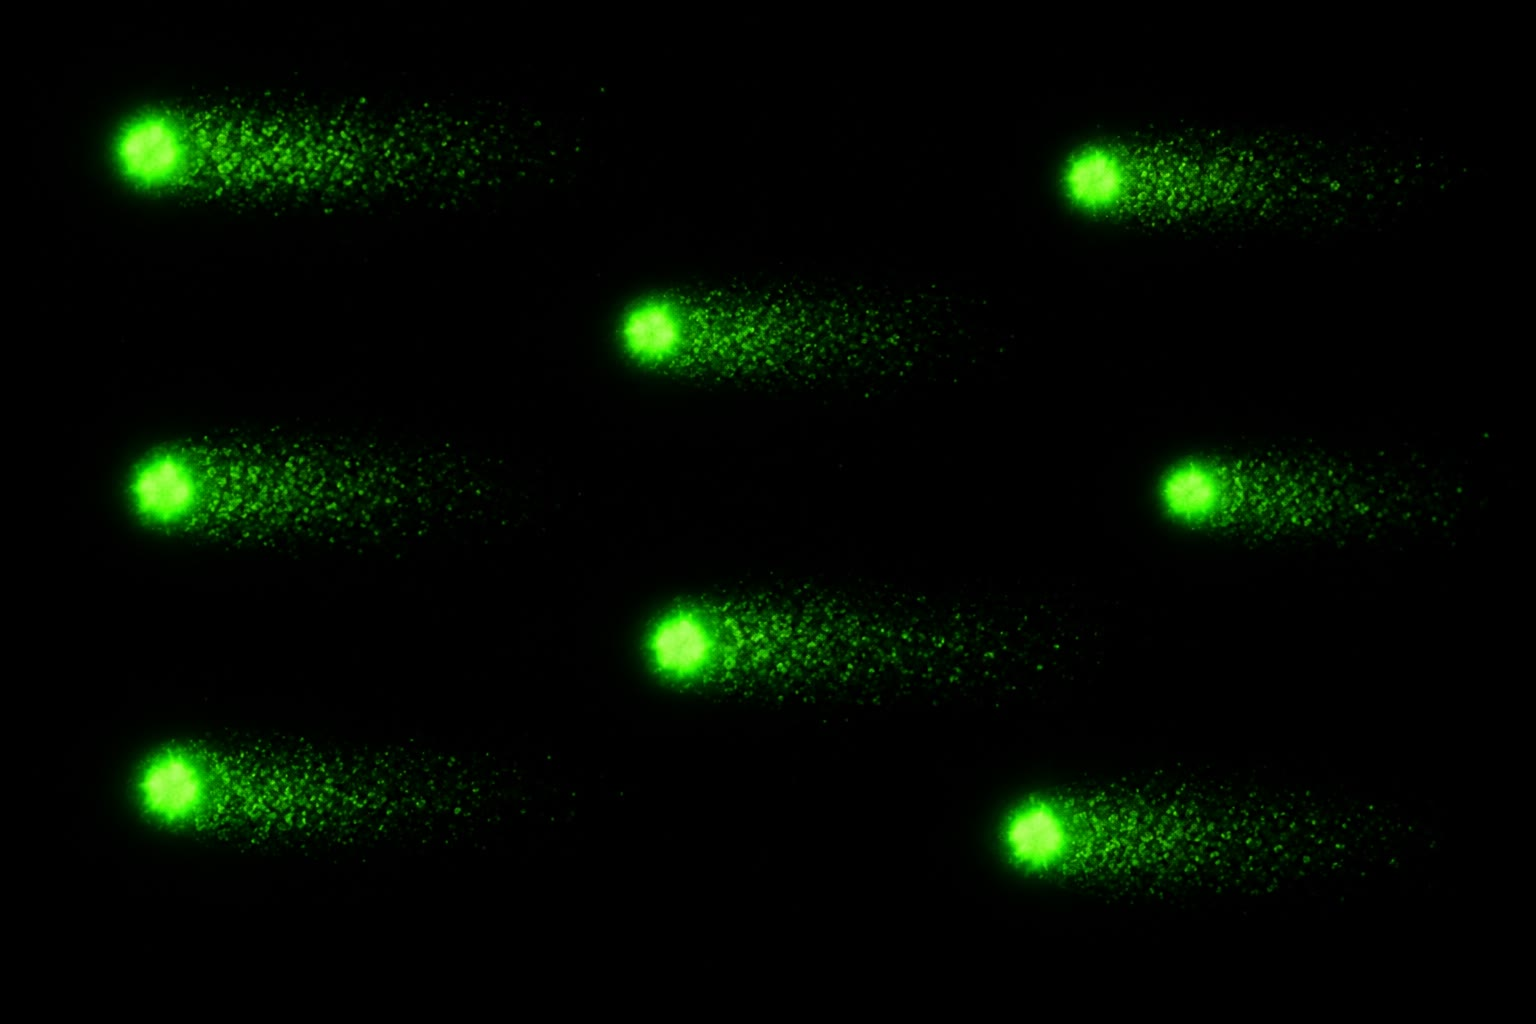
\includegraphics[width=0.46\linewidth]{images/book5/ai/b5-03-comet-assay.jpg}

{\small Kiri: \emph{E.~coli} sesudah penyinaran ultraungu, yang tumbuh
menjadi filamen panjang karena \omterm{prop:b3:dna-repair:sos}{tanggapan SOS} telah menghalangi pembelahan
selnya selama DNA-nya diperbaiki. Kanan: uji komet --- sel tunggal yang
dibenamkan di dalam gel lalu dielektroforesis; DNA yang terpecah mengalir
keluar dari nukleusnya menjadi ekor yang panjangnya mengukur cacah putusnya.}
\end{omfigure}

\begin{definition}[Tanggapan kerusakan DNA]\label{def:b3:dna-repair:ddr}
\index{tanggapan kerusakan DNA}\index{ATM}\index{titik periksa}%
\index{p53}\index{gamma-H2AX}
Eukariot mengisyaratkan kerusakan lewat dua kinase: \emph{ATM}, yang direkrut
kompleks MRN ke \omterm{def:b3:dna-repair:lesions}{putus untai ganda}, dan \emph{ATR}, yang direkrut ke DNA
beruntai tunggal garpu yang terhenti. Keduanya memfosforilasi ratusan
sasaran. Dalam hitungan menit \omterm{def:b3:chromatin-epigenetics:nucleosome}{histon} H2AX terfosforilasi
(\emph{$\gamma$-H2AX}) sepanjang megabasa di sekeliling tiap putus, sehingga
terbentuk fokus yang merekrut protein perbaikan dan dapat dihitung di bawah
mikroskop, satu fokus tiap putus. Kinase Chk1 dan Chk2 menghentikan daur
selnya --- \emph{titik periksa} \cref{ch:b3:cell-cycle-apoptosis} ---
dengan menonaktifkan fosfatase yang akan mendorong masuknya sel ke fase S
atau M; dan faktor transkripsi \emph{p53}, yang dimantapkan oleh
fosforilasi, mengimbas penghambat kinase bergantung-siklin p21 (penghentian
yang awet pada G1), gen perbaikan, dan, bila kerusakannya berat atau
bertahan, gen apoptosis yang membunuh sel itu. Tanggapannya membeli
waktu bagi perbaikan, dan ketika perbaikannya gagal ia menyingkirkan sel itu
alih-alih membiarkannya membelah dengan genom yang putus.
\end{definition}

\begin{omfigure}
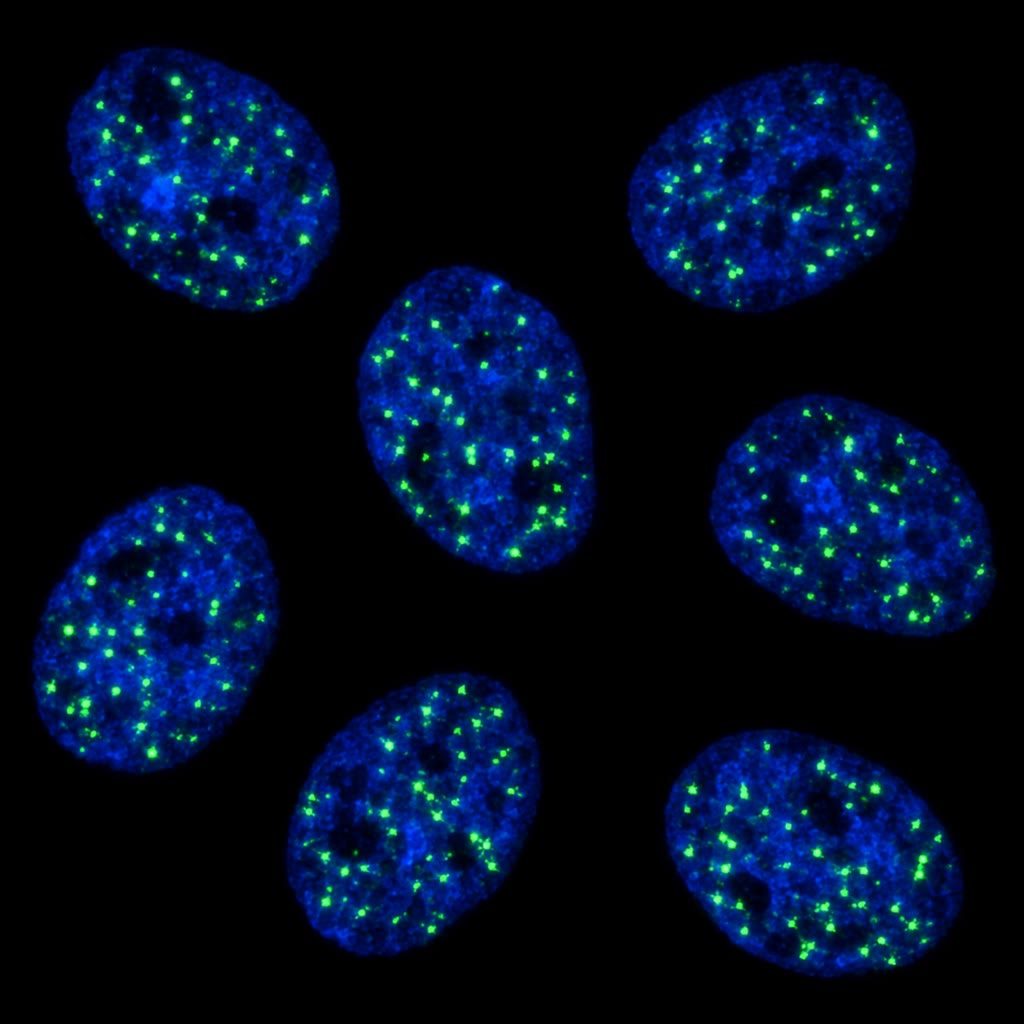
\includegraphics[width=0.4\linewidth]{images/book5/ai/b5-03-gamma-foci.jpg}

{\small Fokus $\gamma$-H2AX (hijau) di dalam nukleus (biru) sejam sesudah
penyinaran. Tiap fokus menandai sebuah \omterm{def:b3:dna-repair:lesions}{putus untai ganda}; menghitungnya
mengukur kerusakannya dan, sepanjang jam-jam berikutnya, perbaikannya.}
\end{omfigure}

\begin{example}[Keletalan sintetik: BRCA dan PARP]\label{ex:b3:dna-repair:parp}
Perempuan yang mewarisi satu salinan cacat \emph{BRCA1} atau \emph{BRCA2}
memiliki risiko kanker payudara seumur hidup sebesar \qtyrange{50}{80}{\%};
tumornya timbul di dalam sel yang telah kehilangan salinan keduanya dan tak
lagi sanggup menjalankan \omterm{def:b3:dna-repair:dsb}{rekombinasi homolog}. Sel semacam itu memperbaiki
\omterm{def:b3:dna-repair:lesions}{putus untai gandanya} dengan penyambungan ujung saja lalu menimbun penataan
ulang. Sel itu juga memperoleh satu kelemahan khas. Putus untai tunggal,
sekitar \num{10000} tiap hari, diperbaiki lewat rute yang menuntut enzim PARP;
ketika PARP dihambat sebuah obat, putus untai tunggalnya bertahan sampai fase
S, dan di situ sebuah garpu mengubah masing-masingnya menjadi \omterm{def:b3:dna-repair:lesions}{putus untai
ganda} berujung satu --- yang hanya dapat diperbaiki rekombinasi. Sel normal,
dengan satu alel \emph{\omterm{def:b3:dna-repair:dsb}{BRCA}} yang baik, sanggup bertahan; sel tumornya mati.
Dua cacat, yang masing-masing tak berbahaya sendirian, mematikan bila
bersama: obatnya membunuh lewat \emph{keletalan sintetik}, dan mengampuni sel
pasien yang lain.
\end{example}

\begin{proposition}[Rekombinasi sebagai alat]\label{prop:b3:dna-repair:tools}
\index{rekombinasi khas tapak}\index{Cre-lox}
Rekombinase khas tapak memotong lalu menyambungkan kembali DNA pada urutan
pendek yang tertentu, tanpa pencarian homologi maupun sintesis: enzim Cre
fag P1 bekerja pada tapak \emph{loxP} sepanjang \qty{34}{bp}, enzim Flp khamir
pada tapak \emph{FRT}. Dua tapak yang searah pada satu molekul mengeksisi DNA
di antaranya sebagai lingkaran; bila berlawanan arah keduanya membalikkannya;
tapak pada dua molekul mempertukarkan sisinya. Sebuah gen yang diapit tapak
\emph{loxP} (``ber-loxP'') dihapus hanya di dalam sel tempat Cre
diekspresikan, dari promotor pilihan peneliti, atau pada waktu yang dipilih
peneliti bila Cre diaktifkan sebuah obat: begitulah gen yang mutlak
diperlukan embrio dikaji pada hati orang dewasa, atau pada neuronnya saja
(\cref{ch:b3:genetic-engineering}). \omterm{def:b3:dna-repair:dsb}{Rekombinasi homolog} milik sel itu
sendirilah yang dipinjam penyasaran gen dan penyuntingan terarah CRISPR untuk
menuliskan urutan pilihan ke tempat pilihan.
\end{proposition}

\begin{remark}[Perbaikan dan penuaan]\label{rem:b3:dna-repair:ageing}
Sel yang gagal memperbaiki menimbun mutasi, menua, atau mati; cacat perbaikan
yang diturunkan (sindrom Werner, sebuah helikase; sindrom Cockayne, perbaikan
yang terkopel transkripsi; ataksia telangiektasia, \omterm{def:b3:dna-repair:ddr}{ATM}) menimbulkan ciri
penuaan dini, dan cacah mutasi somatik jaringan normal naik secara lurus
dengan umur pada laju beberapa puluh mutasi tiap sel tiap tahun. Apakah
kerusakan yang tertimbun \emph{menyebabkan} penuaan biasa, atau sekadar
menyertainya, belum terjawab; bahwa kemampuan memperbaiki adalah salah satu
penentu rentang hidup antarspesies --- spesies yang berumur lebih panjang
memperbaiki lebih banyak --- telah didukung dengan baik.
\end{remark}

\section{Latihan}

\begin{exercise}[$\star$]\label{exo:b3:dna-repair:1}
Golongkanlah \omterm{def:b3:dna-repair:lesions}{lesi} berikut sebagai spontan atau lingkungan lalu sebutkan
jalur perbaikannya masing-masing: sebuah urasil di dalam DNA; sebuah dimer
timina; sebuah \omterm{def:b3:dna-repair:lesions}{8-oksoguanina}; sebuah salah pasang G--T di belakang garpu;
sebuah \omterm{def:b3:dna-repair:lesions}{putus untai ganda} pada G1.
\end{exercise}

\begin{exercise}[$\star$]\label{exo:b3:dna-repair:2}
Mengapa \omterm{def:b3:dna-repair:excision}{perbaikan eksisi nukleotida} tidak menuntut enzim khusus bagi tiap
macam \omterm{def:b3:dna-repair:lesions}{lesi}, sedangkan \omterm{def:b3:dna-repair:excision}{perbaikan eksisi basa} menuntut satu \omterm{def:b3:dna-repair:excision}{glikosilase} bagi
masing-masing?
\end{exercise}

\begin{exercise}[$\star$]\label{exo:b3:dna-repair:3}
Nyatakanlah masalah pembedaan untai pada \omterm{prop:b3:dna-repair:fidelity}{perbaikan salah pasang} dan cara
\emph{E.~coli} memecahkannya. Apa yang akan terjadi pada mutan \emph{dam},
yang tidak memetilasi tapak GATC mana pun?
\end{exercise}

\begin{exercise}[$\star$]\label{exo:b3:dna-repair:4}
Sebuah sel menerima sinar-X sebesar \qty{2}{Gy}. Berapa \omterm{def:b3:dna-repair:lesions}{putus untai ganda}
yang dideritanya, kira-kira, dan berapa fokus $\gamma$-H2AX yang Anda
harapkan terhitung sejam kemudian? Mengapa lebih sedikit sesudah enam jam?
\end{exercise}

\begin{exercise}[$\star\star$]\label{exo:b3:dna-repair:5}
Dengan \cref{prop:b3:dna-repair:fidelity}, hitunglah laju mutasi tiap
pasangan basa dan cacah mutasi baru tiap genom diploid tiap pembelahan pada
(a) sel normal, (b) sel yang kekurangan \omterm{prop:b3:dna-repair:fidelity}{perbaikan salah pasang}, (c) sel yang
polimerasenya kehilangan eksonukleasenya. Mana yang menjadi mutator yang
lebih berbahaya?
\end{exercise}

\begin{exercise}[$\star\star$]\label{exo:b3:dna-repair:6}
Tapak tanpa basa timbul pada $10^{4}$ tiap sel tiap hari dan diperbaiki
dengan waktu paruh \qty{15}{min}. Pakailah \cref{thm:b3:dna-repair:load}
untuk mencari cacah tunak tapak tanpa basa di dalam sebuah sel. Bila sebuah
obat memperlambat perbaikannya sepuluh kali lipat, berapa keadaan tunaknya
yang baru, dan berapa tapak yang akan dijumpai sebuah garpu bila ia menyalin
genomnya dalam \qty{8}{h}?
\end{exercise}

\begin{exercise}[$\star\star$]\label{exo:b3:dna-repair:7}
Pada G2 sebuah putus dapat diperbaiki NHEJ (waktu paruh \qty{30}{min}) atau
HR (waktu paruh \qty{4}{h}), keduanya tersedia. Berapa bagian putus yang
lewat HR? Berapa waktu paruh putusnya? Mengapa HR toh menjadi jalur yang
penting pada garpu replikasi yang runtuh?
\end{exercise}

\begin{exercise}[$\star\star$]\label{exo:b3:dna-repair:8}
Ramalkanlah perilaku mikrosatelit, jangkauan tumor, dan kepekaan terhadap
cahaya matahari seorang pasien dengan (a) \omterm{def:b3:dna-repair:mmr}{sindrom Lynch}, (b)
\omterm{def:b3:dna-repair:excision}{xeroderma pigmentosum} golongan~A, (c) varian XP-V yang tak memiliki
Pol~$\eta$.
\end{exercise}

\begin{exercise}[$\star\star$]\label{exo:b3:dna-repair:9}
Dua tapak \emph{loxP} yang searah mengapit ekson~3 sebuah gen;
Cre diekspresikan dari promotor yang hanya aktif di hati sejak lahir.
Uraikanlah genotipe sel hati dan neuron pada hewan dewasa, dan apa yang
terjadi bila tapaknya justru ditempatkan berlawanan arah.
\end{exercise}

\begin{exercise}[$\star\star\star$]\label{exo:b3:dna-repair:10}
Jelaskanlah mengapa \omterm{prop:b3:dna-repair:sos}{tanggapan SOS} menyalakan gen perbaikan sebelum
polimerase rawan galat, dengan memakai kegemaran LexA pada operatornya, dan
mengapa bakteri yang sama sekali tak memiliki polimerase rawan galat toh
mungkin berada pada posisi yang merugikan di dalam tubuh pasien yang diobati
antibiotik.
\end{exercise}

\begin{exercise}[$\star\star\star$]\label{exo:b3:dna-repair:11}
Sebuah penghambat PARP membunuh sel tumor yang kekurangan \emph{\omterm{def:b3:dna-repair:dsb}{BRCA}} tetapi
tidak membunuh sel normal pasiennya. Paparkanlah rantai sebab-akibatnya, lalu
ramalkan dua cara sebuah tumor dapat menjadi kebal terhadap obat itu dan
bagaimana Anda akan mendeteksi masing-masing.
\end{exercise}

\begin{exercise}[$\star\star\star$]\label{exo:b3:dna-repair:12}
Konversi gen pada sebuah pindah silang memberi tetrad $3{:}1$. Gambarkanlah
(atau uraikanlah) sebuah \omterm{def:b3:dna-repair:dsb}{sambungan Holliday} dengan heterodupleks yang
membentang melintasi sebuah penanda, lalu tunjukkan bagaimana \omterm{prop:b3:dna-repair:fidelity}{perbaikan salah
pasang} heterodupleks itu ke satu arah memberi $3{:}1$, ke arah yang lain
$1{:}3$, dan tanpa perbaikan memberi spora yang dirinya sendiri heterozigot
(pemilahan pascameiosis). Mengapa konversinya terbatas pada penanda yang dekat
dengan pindah silang?
\end{exercise}

\section{Soal: Sehari dalam Hidup Sebuah Genom}

\begin{problem}[{Soal akhir pekan --- kerusakan harian satu sel manusia
yang dihitung, tangga kesetiaan yang dikalikan, sedosis cahaya matahari yang
diikuti sampai ke garpu pada sel normal dan sel yang perbaikannya cacat,
sedosis sinar-X yang dibagi di antara dua jalur perbaikan, dan kelemahan
sebuah tumor yang diubah menjadi obat, berakhir pada cacah dimer yang
dijumpai garpunya, laju mutasi tiap basa, dan bagian putus yang diperbaiki
rekombinasi}]
\label{pb:b3:dna-repair:1}
Data: sebuah sel manusia diploid memiliki $6.4\times 10^{9}$ bp, dan
\qty{1.5}{\%} di antaranya penyandi protein. Kerusakan spontan tiap hari:
$10^{4}$ \omterm{def:b3:dna-repair:lesions}{depurinasi}, $400$ \omterm{def:b3:dna-repair:lesions}{deaminasi} sitosina, $10^{4}$ putus untai
tunggal. Kesetiaan: polimerasenya $10^{-5}$, \omterm{prop:b3:dna-repair:fidelity}{uji bacanya} menyisakan
$10^{-2}$ galat, \omterm{prop:b3:dna-repair:fidelity}{perbaikan salah pasangnya} $10^{-3}$. Sekali berjemur
meninggalkan $10^{5}$ \omterm{def:b3:dna-repair:lesions}{dimer pirimidina} tiap sel kulit; perbaikan eksisinya
berwaktu paruh \qty{2}{h} pada keadaan normal dan \qty{70}{h} pada \omterm{def:b3:dna-repair:excision}{xeroderma
pigmentosum}; sebuah garpu tiba \qty{8}{h} kemudian; pelangkahan sebuah dimer
oleh \omterm{def:b3:dna-repair:tls}{sintesis lintas lesi} menimbulkan mutasi dengan peluang $10^{-3}$.
Sinar-X menghasilkan $35$ \omterm{def:b3:dna-repair:lesions}{putus untai ganda} tiap gray; waktu paruh NHEJ
\qty{30}{min}, waktu paruh HR \qty{4}{h}.

\medskip
\noindent\textbf{Bagian I --- Hari-hari biasa.}
\begin{enumerate}
  \item Berapa \omterm{def:b3:dna-repair:lesions}{lesi} spontan yang diderita sel itu tiap hari,
        dan tiap tahun? Bandingkanlah dengan ukuran genomnya.
  \item Hitunglah laju mutasi tiap pasangan basa tiap pembelahan, dan
        harapan cacah mutasi baru tiap pembelahan.
  \item Berapa banyak di antaranya yang jatuh pada urutan penyandi protein?
        Sepanjang kira-kira $50$ pembelahan dari zigot sampai sel kulit
        dewasa, berapa mutasi penyandi yang diusung sebuah sel kulit dari
        replikasi saja?
  \item Sebuah sel yang kekurangan \omterm{prop:b3:dna-repair:fidelity}{perbaikan salah pasang}: berapa laju
        mutasinya dan berapa mutasi tiap pembelahan? Sebuah mikrosatelit
        tergelincir sekali tiap $10^{4}$ pembelahan tanpa \omterm{prop:b3:dna-repair:fidelity}{perbaikan salah
        pasang} dan sekali tiap $10^{7}$ dengan perbaikan itu. Di dalam
        tumor berisi $10^{9}$ sel yang terbentuk lewat $40$ pembelahan,
        berapa sel yang mengusung alel tergelincir pada mikrosatelit
        tertentu pada tiap kasus? (Taksirlah dengan laju $\times$
        pembelahan $\times$ sel.)
  \item \omterm{def:b3:dna-repair:lesions}{Deaminasi} sitosina memberi urasil, \omterm{def:b3:dna-repair:lesions}{deaminasi} 5-metilsitosina
        memberi timina. Mana yang diperbaiki, oleh apa, dan mana yang
        menjadi mutasi? Kaitkanlah dengan kekurangan \omterm{def:b3:chromatin-epigenetics:methylation}{CpG} pada
        \cref{ch:b3:chromatin-epigenetics}.
  \item Sebuah guanina teroksidasi (8-oksoG) berpasangan dengan A selama
        replikasi. Sel itu memiliki \omterm{def:b3:dna-repair:excision}{glikosilase} bagi 8-oksoG yang
        berhadapan dengan C, \omterm{def:b3:dna-repair:excision}{glikosilase} lain bagi A yang berhadapan
        dengan 8-oksoG, serta hidrolase yang memusnahkan dGTP teroksidasi.
        Jelaskanlah apa yang dicegah masing-masing dan mutasi apa yang
        timbul ketika ketiganya gagal.
\end{enumerate}

\medskip
\noindent\textbf{Bagian II --- Sehari di bawah matahari.}
\begin{enumerate}[resume]
  \item Hitunglah tetapan laju eksisi $k$ bagi sel normal dan sel
        XP.
  \item Berapa dimer yang tersisa pada garpunya pada masing-masing?
  \item Berapa mutasi yang ditimbulkan berjemur itu tiap sel pada
        masing-masing kasus, dan berapa di antaranya yang berada pada
        urutan penyandi?
  \item Sepanjang masa kanak-kanak berisi $500$ paparan semacam itu,
        berapa mutasi penyandi tiap sel kulit pada masing-masing kasus?
        Bandingkanlah dengan cacah dari replikasi saja pada pertanyaan 3.
  \item Sekitar $20$ gen, yang seluruhnya berjumlah \qty{40}{kb} urutan
        penyandi, dapat memacu kanker kulit bila termutasi. Berapa
        peluangnya, tiap sel, bahwa sedikitnya satu mutasi imbasan
        berjemur jatuh pada salah satu gen itu, pada anak XP? (Pakailah
        Poisson dengan rata-rata yang tepat.) Dengan $10^{9}$ sel yang
        terpapar, berapa yang terkena?
  \item Jelaskanlah mengapa masalah sel XP adalah masalah garpunya, bukan
        masalah \omterm{def:b3:dna-repair:lesions}{lesinya} sendiri, dan mengapa kankernya hanya muncul di kulit.
\end{enumerate}

\medskip
\noindent\textbf{Bagian III --- Sedosis sinar-X.}
\begin{enumerate}[resume]
  \item Sebuah dosis \qty{2}{Gy}: berapa \omterm{def:b3:dna-repair:lesions}{putus untai ganda}, dan berapa
        fokus $\gamma$-H2AX sesudah sejam bila NHEJ satu-satunya jalur
        (sel G1)?
  \item Pada sel G2 kedua jalur bekerja. Hitunglah tetapan lajunya
        dan bagian putus yang diperbaiki HR.
  \item Berapa waktu paruh putusnya pada G2, dan berapa yang tersisa
        sesudah sejam?
  \item Tiap peristiwa NHEJ mengubah beberapa pasangan basa pada
        sambungannya. Bila sebuah sambungan jatuh pada urutan penyandi
        dengan peluang $0.015$ dan perubahannya lalu merusak gennya dengan
        peluang $0.7$, berapa gen yang dirusak dosis \qty{2}{Gy} itu tiap
        sel G1?
  \item Dengan $n$ putus serentak, ujungnya dapat tersambung keliru
        menjadi sebuah translokasi. Andaikan tiap pasangan dari $n(n-1)/2$
        pasangan putus tersambung keliru dengan peluang $3\times 10^{-4}$.
        Berapa harapan cacah translokasi tiap sel pada \qty{2}{Gy}? Pada
        \qty{0.2}{Gy}? Mengapa risikonya berskala dengan kuadrat dosisnya
        sedangkan cacah putusnya berskala lurus?
  \item Dosis \qty{2}{Gy} yang sama diberikan sepanjang \qty{10}{h}
        alih-alih sekaligus: berapa putus yang hadir pada satu saat
        (keadaan tunak, NHEJ)? Apa yang tersirat dari hal itu bagi
        translokasi, dan bagi kebiasaan memecah radioterapi menjadi
        beberapa penggal?
  \item Sebuah sel bertahan pada dosis $D$ dengan peluang $e^{-D/D_{0}}$,
        dengan $D_{0} = \qty{1.5}{Gy}$ bagi sel yang perbaikannya utuh dan
        \qty{0.5}{Gy} bagi sel yang tak memiliki NHEJ. Hitunglah ketahanan
        masing-masing pada \qty{2}{Gy} dan pada \qty{6}{Gy}, lalu tafsirkan
        $D_{0}$.
\end{enumerate}

\medskip
\noindent\textbf{Bagian IV --- Kelemahan sang tumor.}
\begin{enumerate}[resume]
  \item Sebuah sel tumor yang kekurangan \emph{BRCA2} memperbaiki putusnya
        dengan NHEJ saja. Dengan pertanyaan 14, berapa bagian putus S/G2-nya
        yang kini diperbaiki secara tak saksama padahal sel normal akan
        memperbaikinya secara saksama? Apa akibatnya bagi genomnya
        sepanjang bertahun-tahun?
  \item Penghambatan PARP meninggalkan $10^{4}$ putus untai tunggal harian
        tanpa perbaikan; \qty{1}{\%} di antaranya diubah garpu menjadi
        \omterm{def:b3:dna-repair:lesions}{putus untai ganda} berujung satu. Berapa putus semacam itu tiap hari
        tiap sel, dan mengapa NHEJ tidak dapat memperbaiki putus berujung
        satu secara benar?
  \item Jelaskanlah mengapa sel normal pasien itu, yang heterozigot untuk
        \emph{BRCA2}, bertahan terhadap obatnya.
  \item Sebuah tumor menjadi kebal lewat mutasi kedua yang memulihkan
        kerangka baca \emph{BRCA2}. Jelaskanlah, lalu katakan bagaimana
        Anda akan mendeteksinya.
  \item Kemoterapi dengan zat pengalkil membunuh sel tumor lewat
        \omterm{prop:b3:dna-repair:fidelity}{perbaikan salah pasang}: enzimnya mencoba memperbaiki basa yang
        teralkilasi lalu memicu kematian sel. Ramalkanlah pengaruh
        obat itu pada tumor \omterm{def:b3:dna-repair:mmr}{sindrom Lynch}, yang tidak memiliki \omterm{prop:b3:dna-repair:fidelity}{perbaikan
        salah pasang}.
  \item Sebutkanlah ketiga hasilnya: dimer yang dijumpai garpu pada sel
        XP (pertanyaan~8), laju mutasi normal tiap pasangan basa
        (pertanyaan~2), dan bagian putus G2 yang diperbaiki HR
        (pertanyaan~14).
\end{enumerate}
\end{problem}
